\section{Сигмоидальный нейрон}

Для решения более сложных задач используются нейроны с непрерывными дифференцируемыми активационными функциями, которые не являются линейными. Один из таких нейронов – сигмоидальный нейрон.

В данной работе хотелось бы, чтобы небольшое изменение в весе вызывало лишь небольшое соответствующее изменение в выходных данных сети. Как будет видно через некоторое время, это свойство сделает обучение возможным. 

Введение функций сигмоидального типа было обусловлено ограниченностью нейронных сетей с пороговой функцией активации нейронов — при такой функции активации любой из выходов сети равен либо нулю, либо единице, что ограничивает использование сетей не в задачах классификации. Использование сигмоидальных функций позволило перейти от бинарных выходов нейрона к аналоговым. Функции передачи такого типа, как правило, 
присущи нейронам, находящимся во внутренних слоях нейронной сети. \\

Сигмоидальный нейрон описывается математически следующим образом: \\

$
  f( \boldsymbol{x}, \boldsymbol{w}, b) = \sigma(\boldsymbol{wx} + b) \\
$

Где $ \mathlarger{\sigma(x) = \frac{1}{1 + e^{-x}}}$  - логистическая функция

\begin{figure}[H]
  \centering
  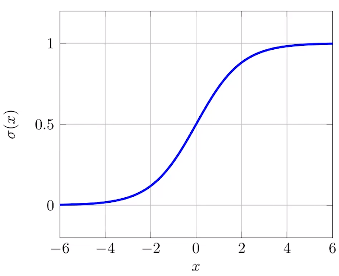
\includegraphics[width=0.5\linewidth]{./img/sigma-func}
  \caption{График логистической функции}
  \label{fig:mpr}
\end{figure} 

Особенностью нейронов с логистической функцией является то, что они усиливают сильные сигналы существенно меньше, чем слабые, поскольку области сильных сигналов соответствуют пологим участкам характеристики. Это позволяет предотвратить насыщение от больших сигналов.

Сигмовидные нейроны похожи на персептроны, но модифицированы так, что небольшие изменения их веса и смещения вызывают только небольшое изменение их выхода. Это решающий факт, который позволит сети сигмовидных нейронов учиться.

\subsection{Квадратичная целевая функция}

$ \mathlarger{ J = \frac{1}{2} \sum_{i=1}^{n} (\hat{y}^{(i)} - y^{(i)}})^2 $ \\
Где $n$ - количество примеров на обучающей выборке \\
$\hat{y}^{(i)} = \sigma (w^T x^{(i)})$ - предсказанное моделью значение \\
$y^{(i)}$ - реальное значение целевой переменной на конкретном примере

Функцией потерь в данном случаю будет выражение $(\hat{y}^{(i)} - y^{(i)})^2$ . В зарубежной литературе функция потерь пишется как \textit{loss function} или \textit{cost function}.
Данная функция была выбрана потому что она проста и понятна. В дальнейшем удобство функции будет заметно при нахождении частных производных. Если взглянуть на функцию внимательно, можно заметить что она зависит от двух аргументов: с одной стороны от данных($\hat{y}^{(i)}$), c другой стороны от параметров модели($y^{(i)}$)